\documentclass[tikz,border=4pt]{standalone}
\usepackage{amsmath,amssymb}
\usetikzlibrary{positioning,arrows.meta,decorations.pathreplacing,calc}

\begin{document}
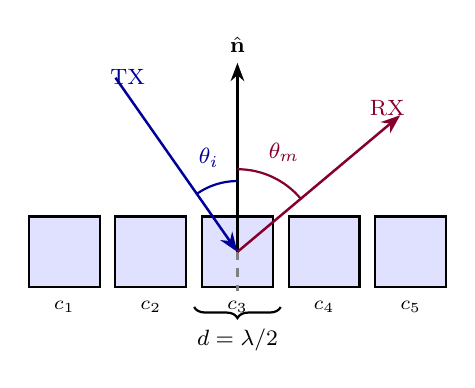
\begin{tikzpicture}[
  >=Stealth, thick, scale=1,
  cell/.style={fill=blue!12, draw=black},
  incray/.style={-{Stealth}, blue!60!black, line width=0.9pt},
  outray/.style={-{Stealth}, purple!70!black, line width=0.9pt},
  normal/.style={-{Stealth}, black, line width=0.8pt},
  every node/.style={font=\footnotesize}
]

  % --- RIS surface: 5 unit cells spaced by d = lambda/2 ---
  \foreach \i/\name in {-2/cm2, -1/cm1, 0/c0, 1/c1, 2/c2} {
    \node[cell, minimum width=0.9cm, minimum height=0.9cm] (\name) at (1.1*\i,0) {};
  }
  \node[below=1pt of cm2] {\scriptsize $c_1$};
  \node[below=1pt of cm1] {\scriptsize $c_2$};
  \node[below=1pt of c0]  {\scriptsize $c_3$};
  \node[below=1pt of c1]  {\scriptsize $c_4$};
  \node[below=1pt of c2]  {\scriptsize $c_5$};

  % spacing d = lambda/2 between two adjacent cells
  \draw[decorate, decoration={brace, amplitude=4pt, mirror}, thick]
        (-0.55,-0.7) -- (0.55,-0.7) node[midway, below=4pt] {$d=\lambda/2$};

  % surface normal at the center cell c3
  \draw[normal] (c0.center) -- ++(0,2.4) node[above] {$\hat{\mathbf n}$};
  \draw[dashed, gray] (c0.center) -- ++(0,-0.5);

  % incident ray from TX side, at angle theta_i from the normal
  \coordinate (src) at ($(c0.center)+(125:2.7)$);
  \draw[incray] (src) -- (c0.center) node[pos=0.1, above, blue!60!black] {TX};
  \draw[blue!60!black] ($(c0.center)+(90:0.9)$) arc (90:125:0.9);
  \node[blue!60!black] at ($(c0.center)+(107:1.25)$) {$\theta_i$};

  % outgoing (reradiated) ray towards RX side, at angle theta_m from the normal
  \coordinate (dst) at ($(c0.center)+(40:2.7)$);
  \draw[outray] (c0.center) -- (dst) node[pos=0.92, above, purple!70!black] {RX};
  \draw[purple!70!black] ($(c0.center)+(40:1.05)$) arc (40:90:1.05);
  \node[purple!70!black] at ($(c0.center)+(65:1.4)$) {$\theta_m$};

\end{tikzpicture}
\end{document}
